
\documentclass[a4paper,12pt]{article}
\usepackage{graphicx}
\usepackage[table,xcdraw]{xcolor}
\usepackage{geometry}
\usepackage{float}
\usepackage[colorlinks=false, hidelinks]{hyperref}
\usepackage{fancyhdr}% For page numbering
\geometry{top=1in,bottom=1in,left=1in,right=1in}
\usepackage{listings}
\usepackage{xcolor}
\usepackage{hyperref}
\pagestyle{empty}
\usepackage{listings}
\usepackage{tcolorbox}

% Define Solarized Light color scheme
\definecolor{base03}{HTML}{002b36}
\definecolor{base02}{HTML}{073642}
\definecolor{base01}{HTML}{586e75}
\definecolor{base00}{HTML}{657b83}
\definecolor{base0}{HTML}{839496}
\definecolor{base1}{HTML}{93a1a1}
\definecolor{base2}{HTML}{eee8d5}
\definecolor{base3}{HTML}{fdf6e3}
\definecolor{yellow}{HTML}{b58900}
\definecolor{orange}{HTML}{cb4b16}
\definecolor{red}{HTML}{dc322f}
\definecolor{magenta}{HTML}{d33682}
\definecolor{violet}{HTML}{6c71c4}
\definecolor{blue}{HTML}{268bd2}
\definecolor{cyan}{HTML}{2aa198}
\definecolor{green}{HTML}{859900}

% Set YAML listing style
\lstdefinelanguage{yaml}{
  morekeywords={true,false,null,y,n,yes,no},
  sensitive=false,
  comment=[l]{\#},
  morecomment=[s]{/*}{*/},
  morestring=[b]',
  basicstyle=\ttfamily,
  breaklines=true,
  columns=fullflexible,
  keepspaces=true,
  escapeinside={(*@}{@*)}
}


\usepackage{listings}
\lstset{
  basicstyle=\ttfamily\small,
  breaklines=true,
  columns=fullflexible,
  keepspaces=true,
  showstringspaces=false,
  language=Yaml, % or 'Bash' for shell commands
}


\begin{document}

\begin{center}
    \textbf{\large{Lab Report: Continous Integration}}\\
    \vspace{0.2cm}
    \textbf{Course Title: Software Engineering \& ISD Lab}\\
    \vspace{0.2cm}
    \textbf{Course Code: CSE-404}\\
    \vspace{0.2cm}
    \textbf{4\textsuperscript{th}Year 1\textsuperscript{st}Semester Examination 2023}\\
    \vspace{0.5cm}
    \textbf{Date of Submission: \today}\\

    \vspace{1.5cm}
    
\includegraphics[width=0.35\textwidth]{images/logo.png}\\ % Replace 'logo.png' with the correct path if you have the university logo image
    \vspace{1cm}

    \textbf{Submitted to}\\
    \vspace{0.2cm}
    \textbf{\href{https://juniv.edu/teachers/musfique.anwar}{Dr. Md Musfique Anwar}}\\
    {Professor}\\
    \vspace{0.2cm}
    \textbf{\href{https://juniv.edu/teachers/hkabir}{Dr. Md. Humayun Kabir}}\\
    {Professor}\\


    \vspace{1cm}

    \begin{table}[h!]
        \centering
        \arrayrulecolor{black}
        \begin{tabular}{|c|c|c|c|}
            \hline
            \rowcolor[HTML]{2F4F4F} % Changed header background color to dark slate gray
            {\color[HTML]{FFFFFF}\textbf{Sl}}& {\color[HTML]{FFFFFF}\textbf{Class Roll}}& {\color[HTML]{FFFFFF}\textbf{Exam Roll}}& {\color[HTML]{FFFFFF}\textbf{Name}}\\ \hline
            \rowcolor[HTML]{B0E0E6}
            \textbf{1}& \textbf{408} & \textbf{202220} & \textbf{Sudipta Singha} \\ \hline
       
        \end{tabular}
    \end{table}

    \vspace{1cm}

    Department of Computer Science and Engineering\\
    Jahangirnagar University\\
    Savar, Dhaka, Bangladesh\\
\end{center}

\newpage

\tableofcontents

\newpage
\pagestyle{fancy}
\fancyhf{}
\fancyfoot[C]{\thepage} % Page number in the center of the footer
\section{Introduction}
Continuous Integration (CI) is a core agile practice aimed at enhancing software development by integrating
code changes frequently, automating builds, and running tests continuously. CI ensures that the codebase
remains functional and deployable at all times, reducing integration problems and accelerating development
cycles. This report captures my individual contributions and reflections on adopting and practicing CI during
our project’s development phase.
\section{Individual Contribution to CI Practice}
\begin{enumerate}
    \item \textbf{Tool Selection}
        \begin{itemize}
            \item After evaluating several CI tools, I recommended the following for the project:
                \begin{itemize}
                    \item Github Actions: For automating the CICD pipeline and to enforce testing and linting before code commits.
                    \item Django Built-in Unit Test Framework: For automating unit and integration tests.
                \end{itemize}
            \item Justification: These tools are open-source, scalable, and compatible with our tech stack.
        \end{itemize}
    \item \textbf{Pipeline Setup}
        \begin{itemize}
            \item Configured Github Actions to:
                \begin{itemize}
                    \item Pull code from the repository upon push events.
                    \item If the testing is passed, we can merge this branch to the main branch
                    \item Build the application in Ubuntu Environment.
                    \item Run automated tests using Django Built-In Test Framework.
                    \item Generate reports for failed tests.
    \end{itemize}
    \item Integrated email notifications to inform the team of build statuses.
\end{itemize}
\item \textbf{Build Automation}
    \begin{itemize}
        \item Created scripts to:
            \begin{itemize}
                \item Automatically install dependencies.
                \item Set up and tear down test databases.
                \item Deploy successful builds to a staging environment for further testing.
\end{itemize}
\end{itemize}
\item \textbf{Documentation and Training}
    \begin{itemize}
        \item Documented the CI setup process, including troubleshooting common issues.
        \item Conducted meeting to familiarize team members with the CI workflow.
\end{itemize}
\end{enumerate}
\textbf{Github Actions cicd.yml}
\begin{tcolorbox}[colback=base3, colframe=base2, sharp corners=all]
\begin{lstlisting}
name: Django CI/CD pipeline
on:
  push:
    branches:
      - main
      - ci-testing-ss
      - ci-testing-sd
  pull_request:
    branches:
      - main
      - ci-testing-ss
      - ci-testing-sd

jobs:
  test:
    runs-on: ubuntu-latest
    steps:
      - name: Checkout code
        uses: actions/checkout@v3

      - name: Set up Python
        uses: actions/setup-python@v4
        with:
          python-version: 3.12.4

      - name: Install dependencies
        run: |
          python -m pip install --upgrade pip
          pip install -r requirements.txt

      - name: Create media directory
        run: |
          mkdir -p jumcms/media

      - name: Set up environment variables
        run: |
          echo "SECRET_KEY=django-insecure-+5@v2_e=w9+%xz3xmr&inw-0c%af4r8e&uu+__0y27x6ysf^o-" >> $GITHUB_ENV
          echo "DEBUG=True" >> $GITHUB_ENV

      - name: Run database migrations
        run: |
          python jumcms/manage.py makemigrations
          python jumcms/manage.py migrate

      - name: Run tests
        run: |
          python jumcms/manage.py test ambulance.tests appointments.tests blogs.tests certifications.tests medical_tests.tests medicines.tests users.tests
\end{lstlisting}
\end{tcolorbox}
\begin{figure}[H]
    \centering
    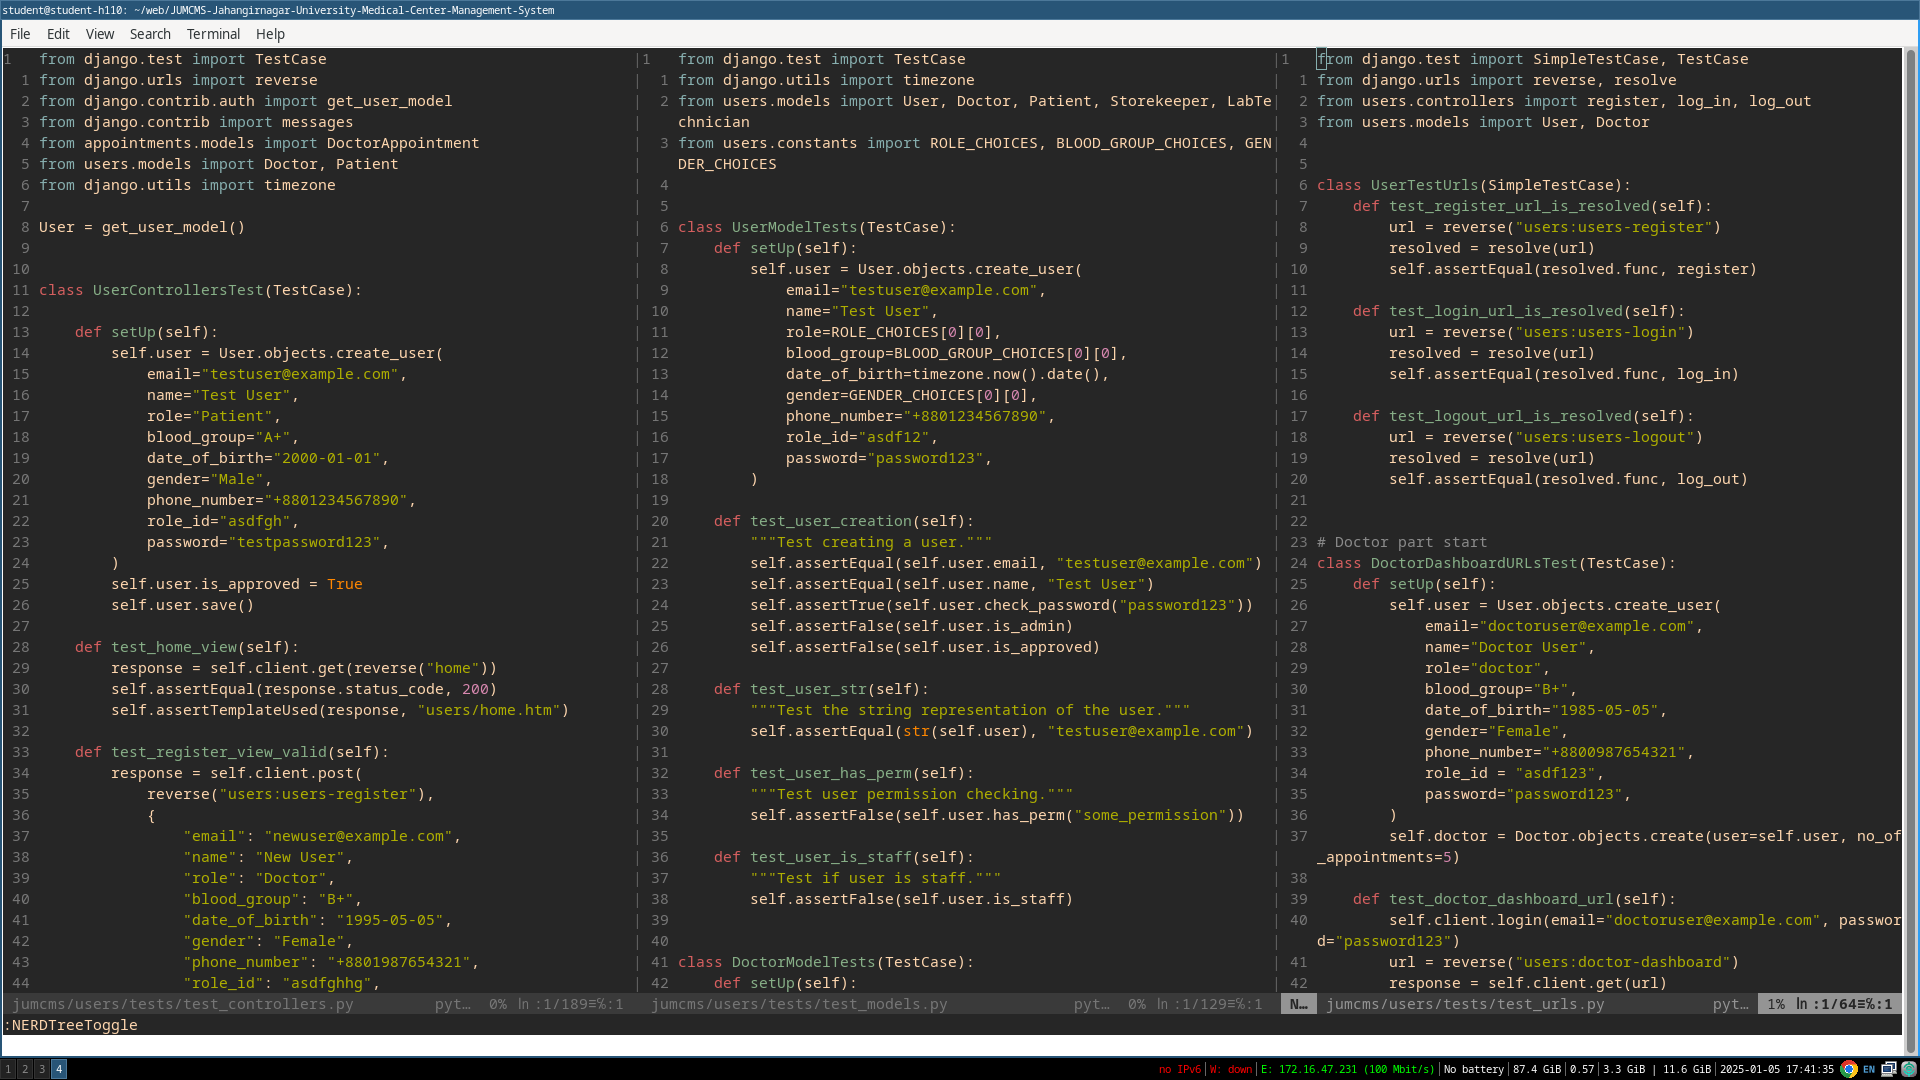
\includegraphics[width=1\textwidth]{images/TDD1.png}
    \caption{Test Code for create account feature}
    \label{fig:tdd1}
\end{figure}
\begin{figure}[H]
    \centering
    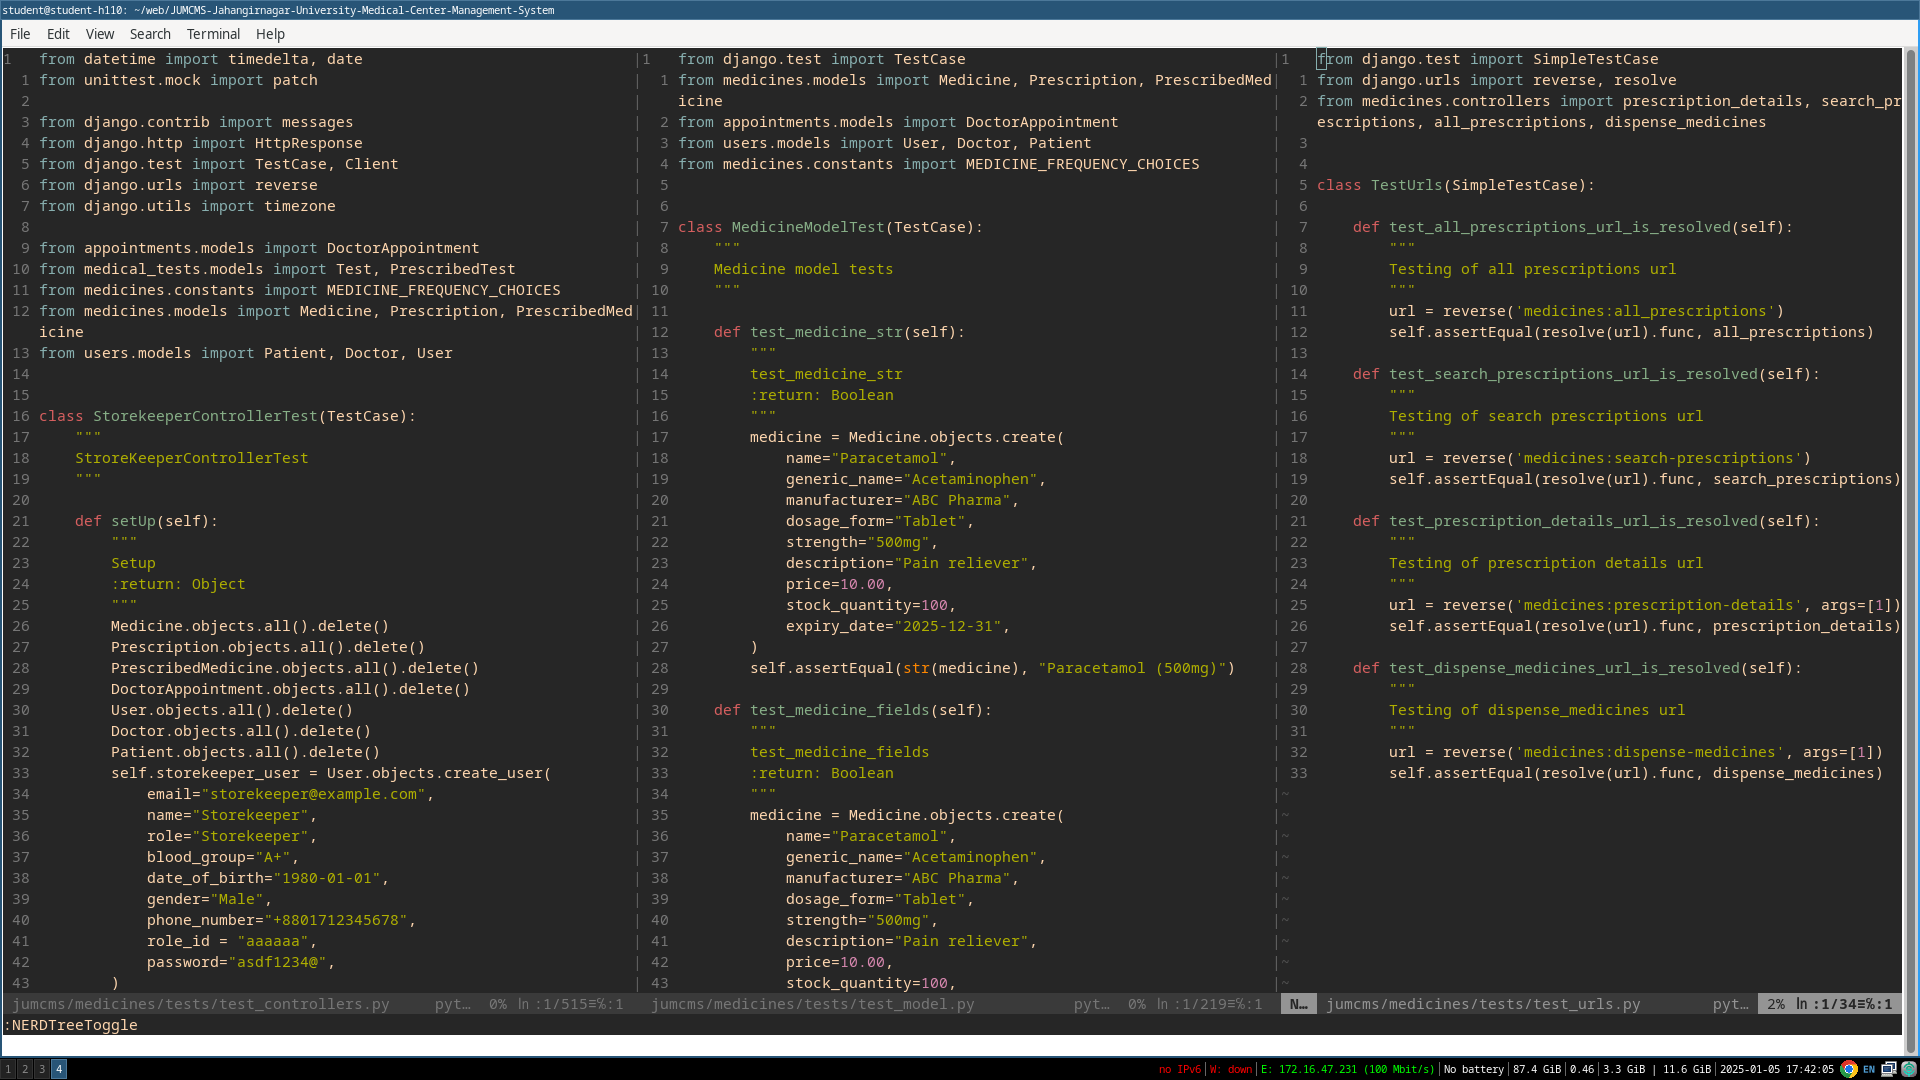
\includegraphics[width=1\textwidth]{images/TDD2.png}
    \caption{Test code for dispense medicine and update stock information feature}
    \label{fig:tdd2}
\end{figure}

\begin{figure}[H]
    \centering
    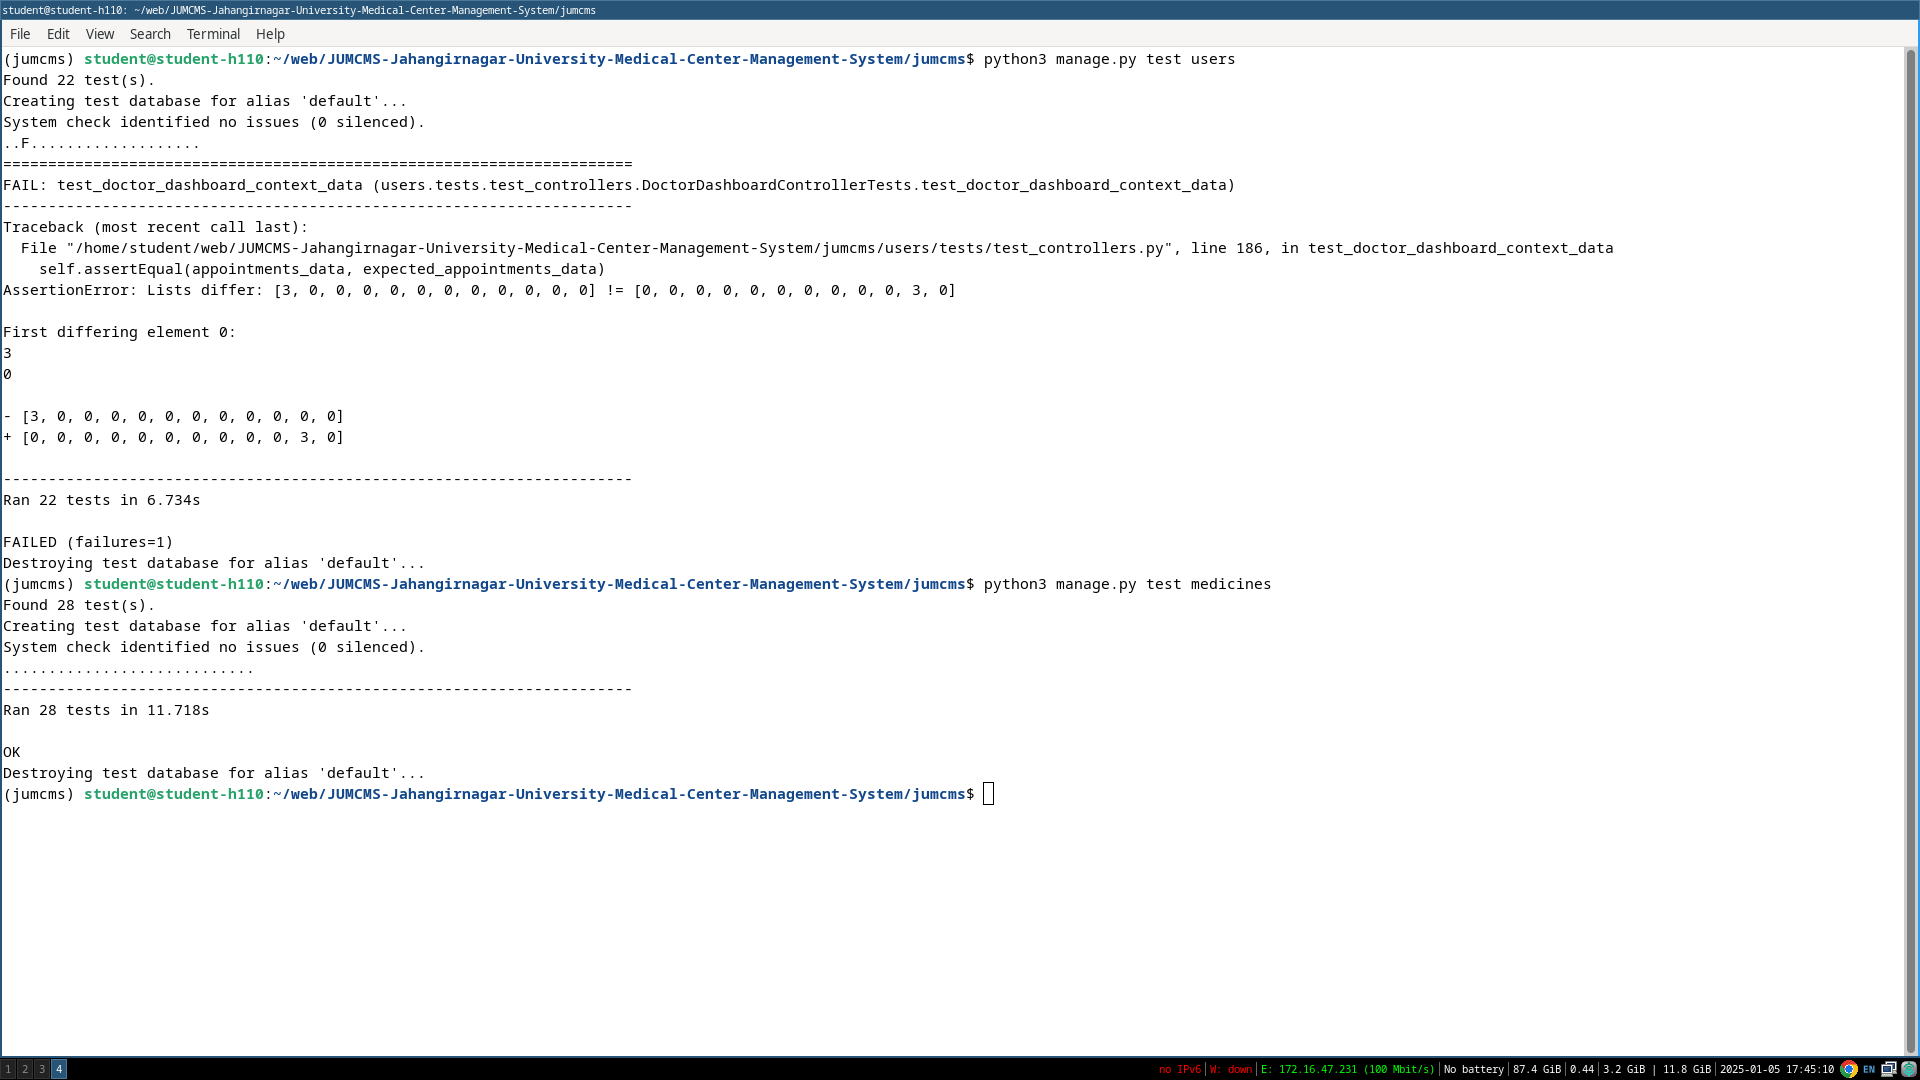
\includegraphics[width=1\textwidth]{images/TDD3.png}
    \caption{Test case result}
    \label{fig:tdd3}
\end{figure}
\begin{figure}[H]
    \centering
    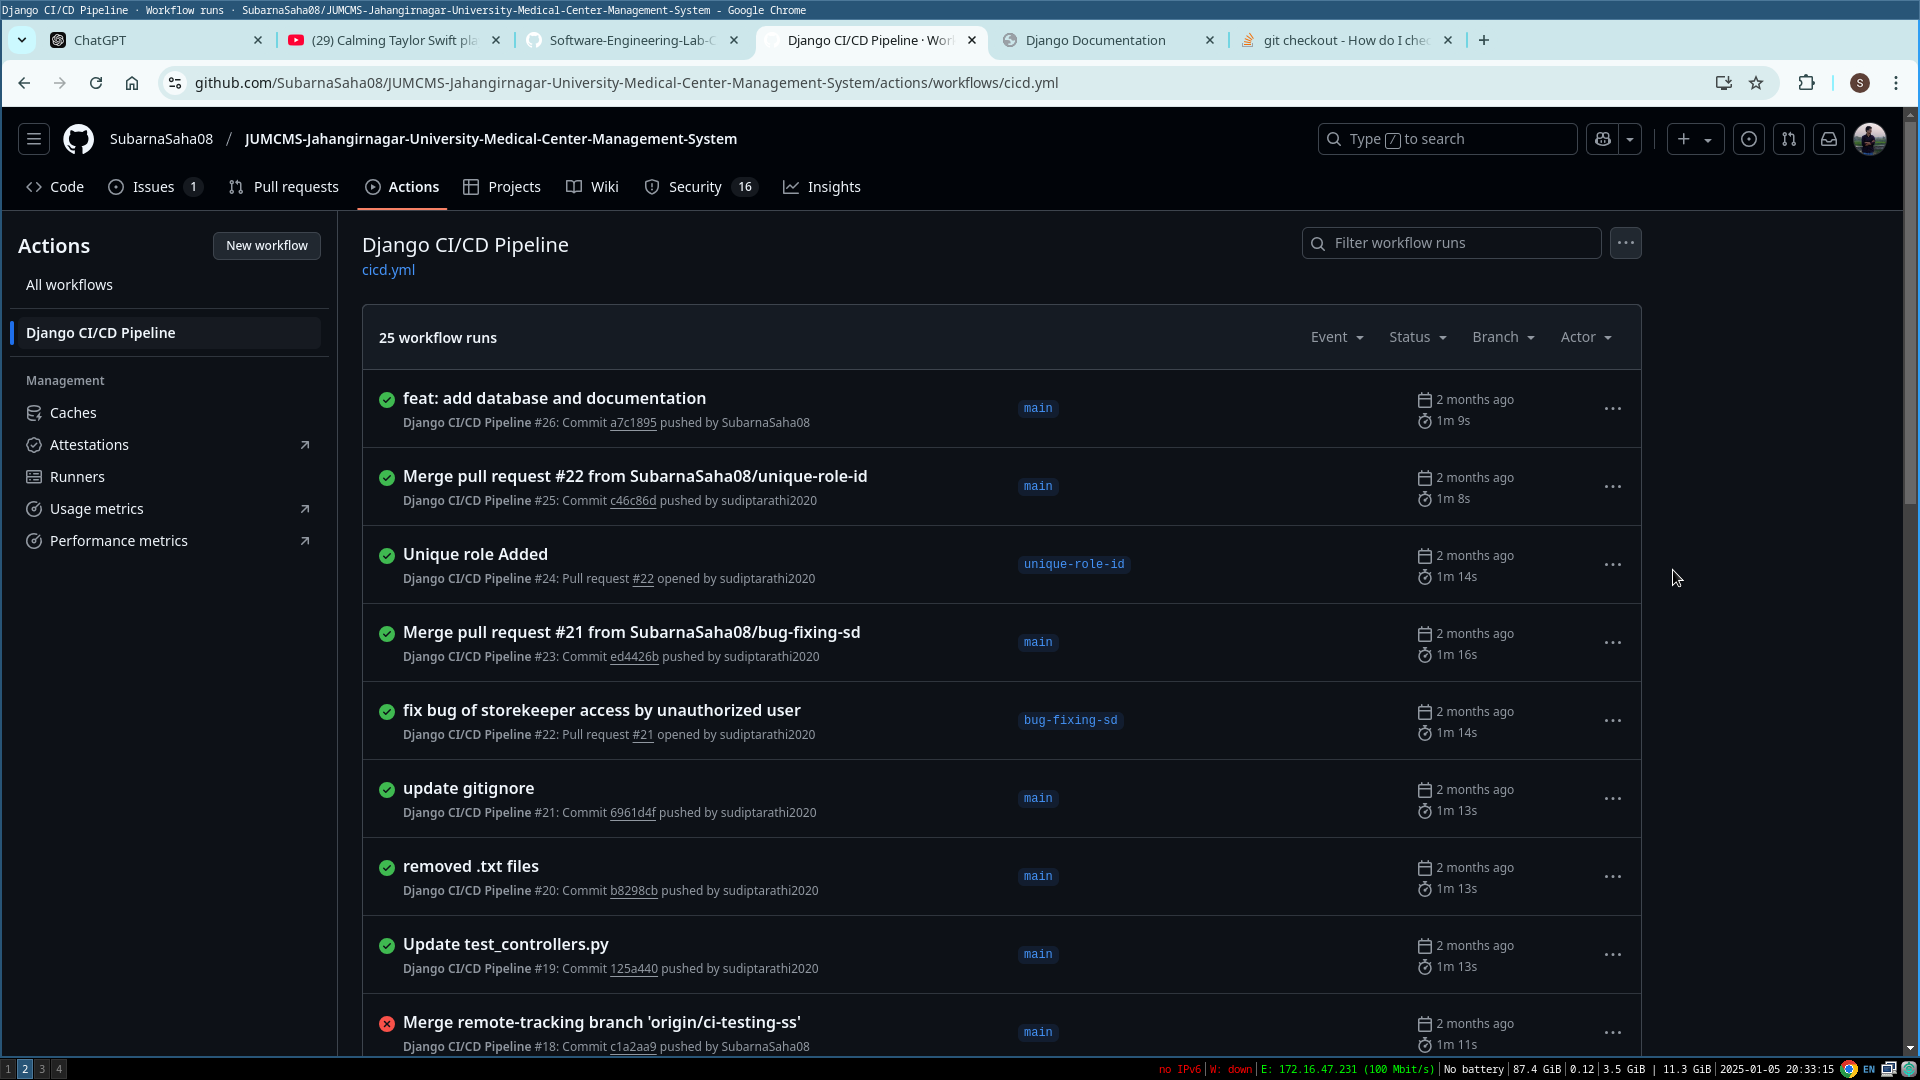
\includegraphics[width=1\textwidth]{images/CI.png}
    \caption{List of github run for pull request}
    \label{fig:ci}
\end{figure}


\begin{figure}[H]
    \centering
    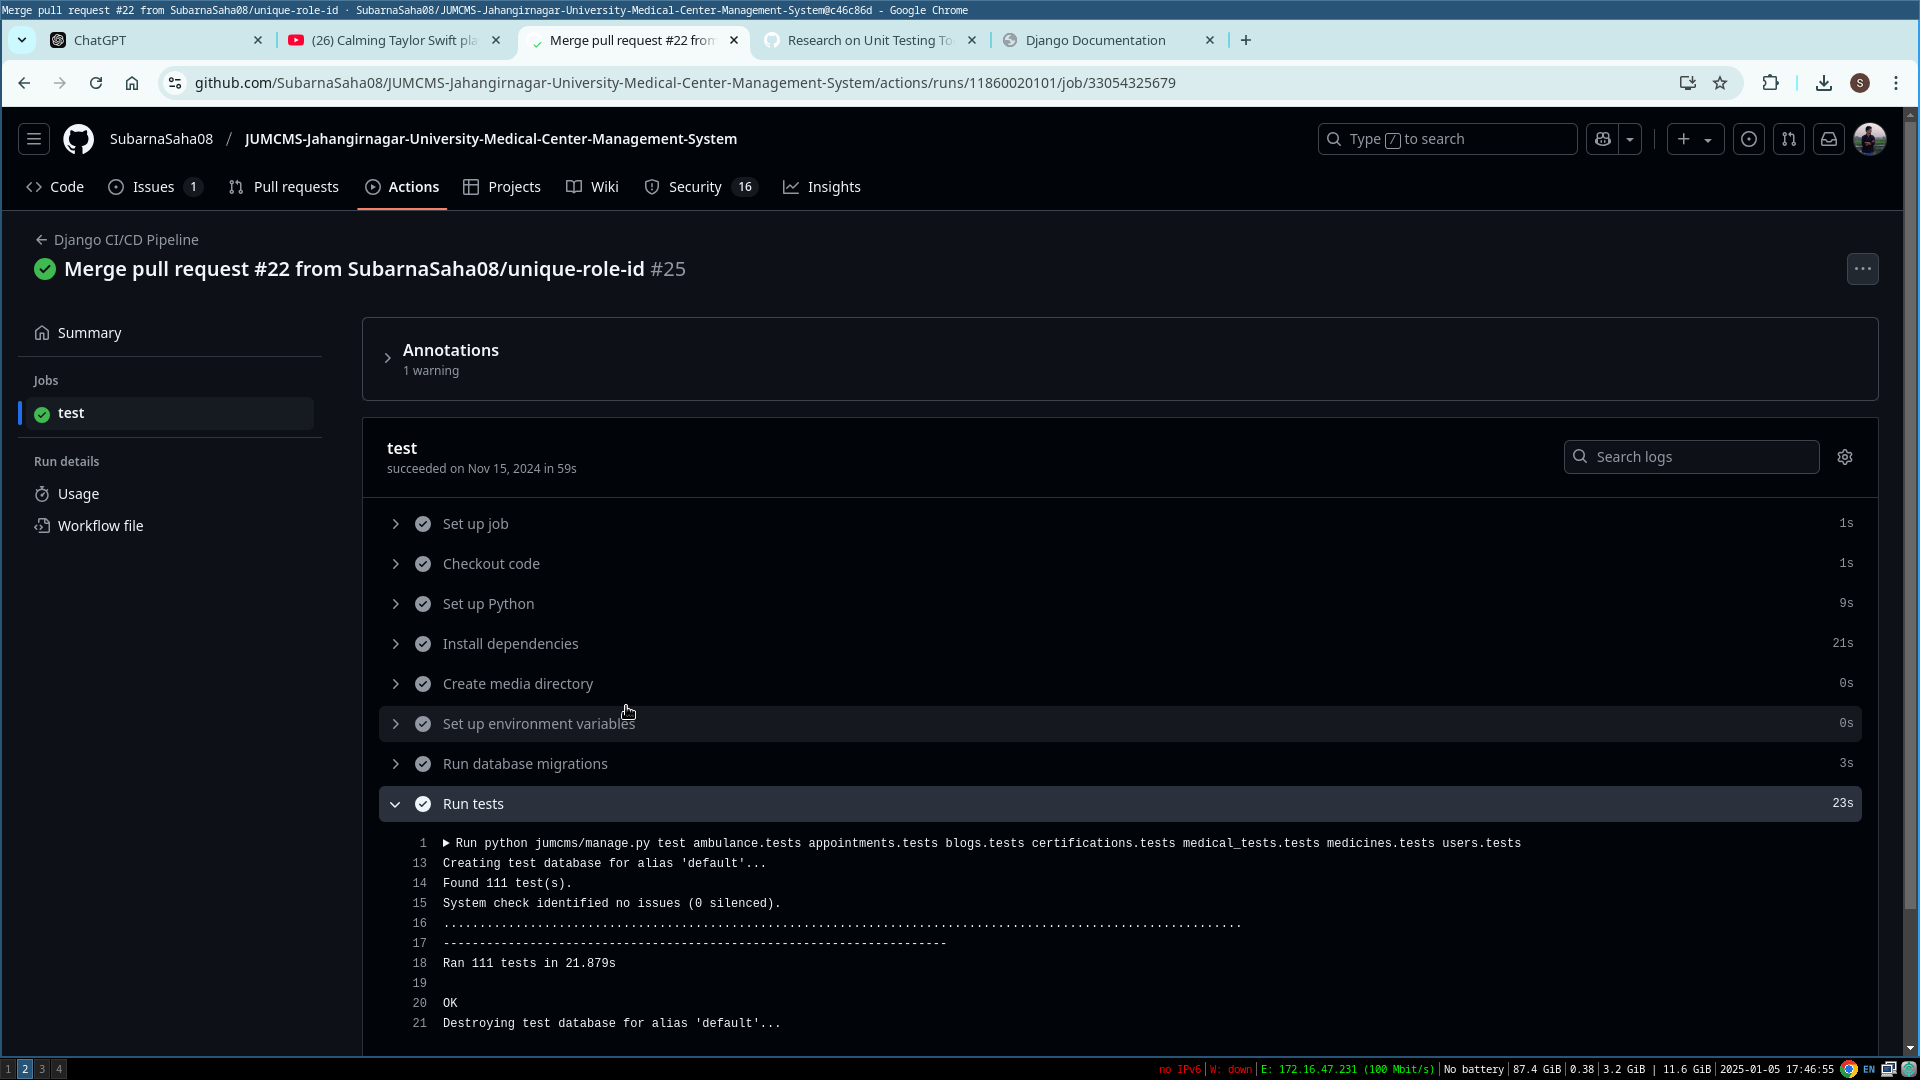
\includegraphics[width=1\textwidth]{images/TDD4.png}
    \caption{YML file running screenshot}
    \label{fig:tdd4}
\end{figure}

\section{Reflection on CI Experience}
\begin{enumerate}
    \item \textbf{Benefits Observed}
        \begin{itemize}
            \item Reduced Integration Issues: Frequent integrations minimized conflicts and ensured early detection of errors.
            \item Faster Feedback Loop: Automated builds and tests provided immediate feedback on code changes.
            \item Improved Team Productivity: Automating repetitive tasks freed up time for development and innovation.
            \item Enhanced Code Quality: Continuous testing ensured that the code adhered to quality standards throughout the development cycle.
\end{itemize}
\item \textbf{Challenges Faced}
    \begin{itemize}
        \item Initial Setup Complexity: Configuring github actions for our project required significant effort.
        \item Flaky Tests: Some tests failed intermittently due to dependency on external services.
        \item Resource Limitations: Running frequent builds and tests strained server resources.
\end{itemize}
\item \textbf{Resolution of Challenges}
    \begin{itemize}
        \item Simplified the CI pipeline by modularizing scripts and prioritizing essential tasks.
        \item Mocked external dependencies in tests to reduce flakiness.
        \item Optimized resource usage by scheduling non-critical builds during off-peak hours.
\end{itemize}
\end{enumerate}
\section{CI’s Impact on Project Outcomes}
\begin{enumerate}
    \item \textbf{Improved Collaboration}
        \begin{itemize}
            \item CI fostered a culture of shared responsibility for the codebase. Developers integrated changes
                frequently, reducing silos and improving team communication.
        \end{itemize}
    \item \textbf{Faster Iterations}
        \begin{itemize}
            \item Automated testing and deployment enabled the team to release incremental updates more
                frequently, accelerating delivery cycles.
    \end{itemize}
\item \textbf{Complementary Practices}
    \begin{itemize}
        \item Test-Driven Development (TDD): CI seamlessly integrated with TDD by running unit tests before
            every build.
        \item Version Control: Git hooks ensured clean commits, making the CI process more efficient.
\end{itemize}
\end{enumerate}
\section{Guidelines for Effective CI Practices}
\begin{enumerate}
    \item \textbf{Automate Everything}
        \begin{itemize}
            \item Automate builds, tests, deployments, and notifications to reduce manual effort and human
                error.
\end{itemize}
\item \textbf{Keep Builds Fast}
    \begin{itemize}
        \item Optimize build scripts and parallelize tasks to maintain a quick feedback loop.
\end{itemize}
\item \textbf{Test Thoroughly}
    \begin{itemize}
        \item Include unit, integration, and regression tests in the CI pipeline to ensure comprehensive
            validation.
\end{itemize}
\item \textbf{Monitor and Maintain}
    \begin{itemize}
        \item Regularly review and update CI configurations to address evolving project needs and challenges.
\end{itemize}
\item \textbf{Foster Team Buy-In}
    \begin{itemize}
        \item Involve the entire team in the CI process to ensure adherence and shared ownership.
\end{itemize}
\end{enumerate}
\section{Conclusion}
Practicing Continuous Integration significantly enhanced our project’s quality and delivery efficiency. While
initial setup required effort, the long-term benefits—including reduced integration issues, faster iterations,
and improved team collaboration—proved invaluable. By combining CI with other agile practices like TDD, our
team successfully delivered a robust and maintainable software solution.
\end{document}
